\section{Tecnología P4}
\label{TecnologiaP4}

La tecnología P4\footnote{\textit{\textbf{P}rogramming \textbf{P}rotocol-independent \textbf{P}acket \textbf{P}rocessors}} se diseñó principalmente como un lenguaje de alto nivel para programar procesadores de paquetes. Su impulso vino de la mano de un consorcio de empresas privadas relacionadas con el mundo de las telecomunicaciones y fabricantes de hardware, conocido como P4 Language Consortium. Más tarde, conforme la tecnología fue ganando fuerza, el proyecto P4 pasó a ser parte de la \gls{onf} ganando así más difusión en la comunidad.\\
\par
Dicha tecnología nació con el propósito de cubrir las limitaciones del protocolo OpenFlow. El protocolo OpenFlow a través de distintas versiones había aumentado la cantidad de campos de cabeceras, admitiendo así más protocolos, pasando de 12 campos a 41 en cuatro años. Este hecho supuso un aumento en la complejidad de la especificación del protocolo, y aún seguían limitados en dar flexibilidad para añadir nuevas cabeceras \cite{2014p4}.\\
\par
Debido a lo cual, se presentaba P4 como una solución hacia donde debía evolucionar OpenFlow. Para ello, se basaron en tres pilares fundamentales, el primero de ellos era conseguir que los dispositivos de red fuera reconfigurables en vuelo, el segundo consistía en que los switches fueran agnósticos a cualquier protocolo de red, y por último, se quería que el lenguaje P4 fuera completamente independiente del hardware sobre el cual se fuera a implantar. 

% Foto elisa 
\begin{figure}[ht]
    \centering
    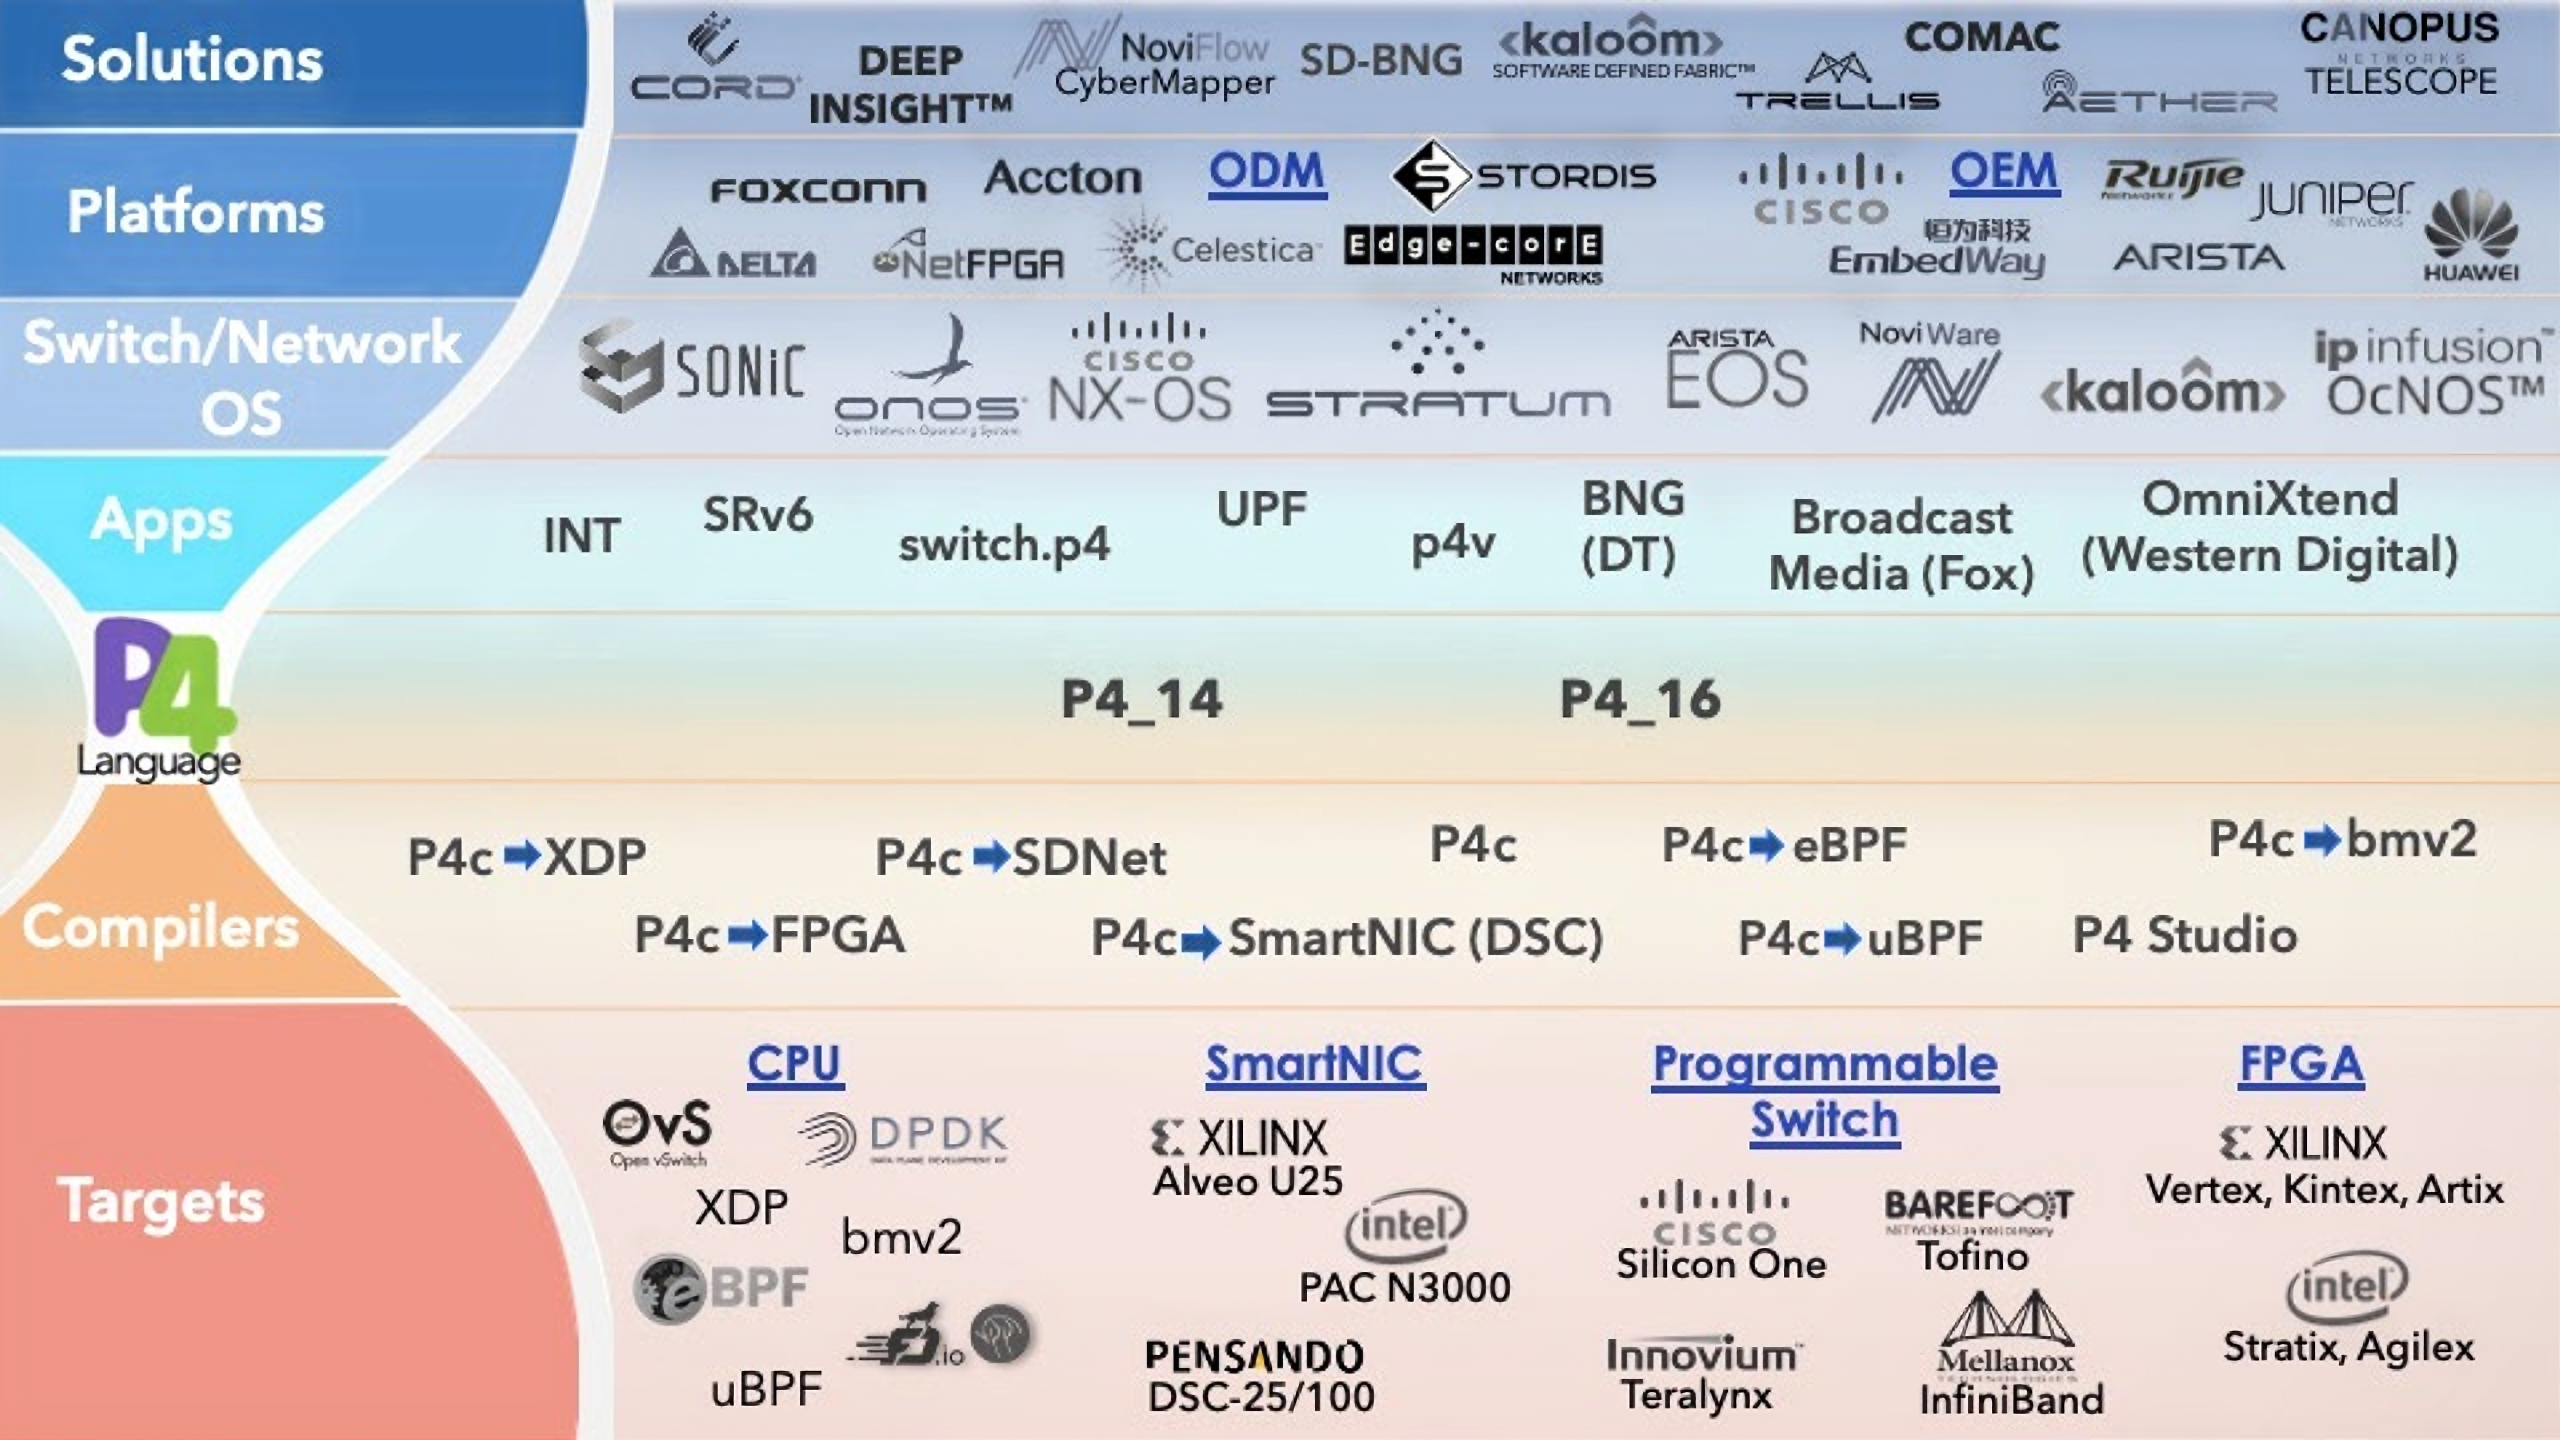
\includegraphics[width=14.5cm]{archivos/img/teoria/p4resumen_edited2.png}
    \caption{Ecosistema P4}
    \label{fig:p4eco}
\end{figure}

A día de hoy la tecnología P4 ya está ampliamente implantada. Como se puede apreciar en la figura \ref{fig:p4eco}, se ha generado todo un ecosistema entorno a esta tecnología, contando con numerosos compiladores de \textit{backend} enfocados para los distintos \textit{targets}, con aplicaciones y soluciones ya puestas en funcionamiento. Por lo que todo apunta a que este ecosistema tiende a ir a más, si bien es verdad que aún tiene ciertas dificultades con ciertos tipos de hardware, pero su futuro es bastante prometedor. 


%%%%%%%%%%%%%%%%%%%%%%%%%%%%%%%%%%%%%%%%%%%%%%%%%%%%%%%%%%%%%%%%%%%%%%%%%%%%%%%%%%%
\subsection{Objetivos}

Por tanto, la llegada de la tecnología P4 supuso una cambio de paradigma a la hora de diseñar nuevos protocolos. Esto es así ya que permitía decir a los \textit{switches} como debían operan en vez de estar limitados por las condiciones de diseño del propio \textit{switch} (Ver figura \ref{fig:p4Paradigma}). Este paradigma se alcanzaría encontrando un termino medio entre la expresividad del lenguaje P4 y la compatibilidad de éste entre la gran mayoría de hardware y soft-switches. Por ello, se plantearon tres hitos a conseguir \cite{2014p4}.

\begin{itemize}
    \item \textbf{Reconfigurabilidad}. En un entorno \gls{sdn}, el controlador debería ser capaz de redefinir el \textit{datapath} de los \textit{switches}.
    \item \textbf{Agnóstico a protocolos}. Los switches no deben tener ningún conocimiento sobre los protocolos de red, es deber del controlador especificar como debe analizar y procesar los paquetes que le lleguen para extraer las cabeceras, y una serie de tablas del tipo \textit{match-action} para procesar esas cabeceras. 
    \item \textbf{Independencia de la arquitectura}. Al igual que los programadores de aplicaciones no tienen que especificar sobre que arquitectura están compilando su aplicación, se quería que los programadores de P4 no se preocuparan sobre en que arquitectura se iba a correr dicho programa P4. Será deber de los compiladores tomar el programa P4 totalmente independiente de arquitectura y convertirlo en un programa que dependa de la arquitectura en cuestión.
\end{itemize}

% Foto 
\begin{figure}[ht]
    \centering
    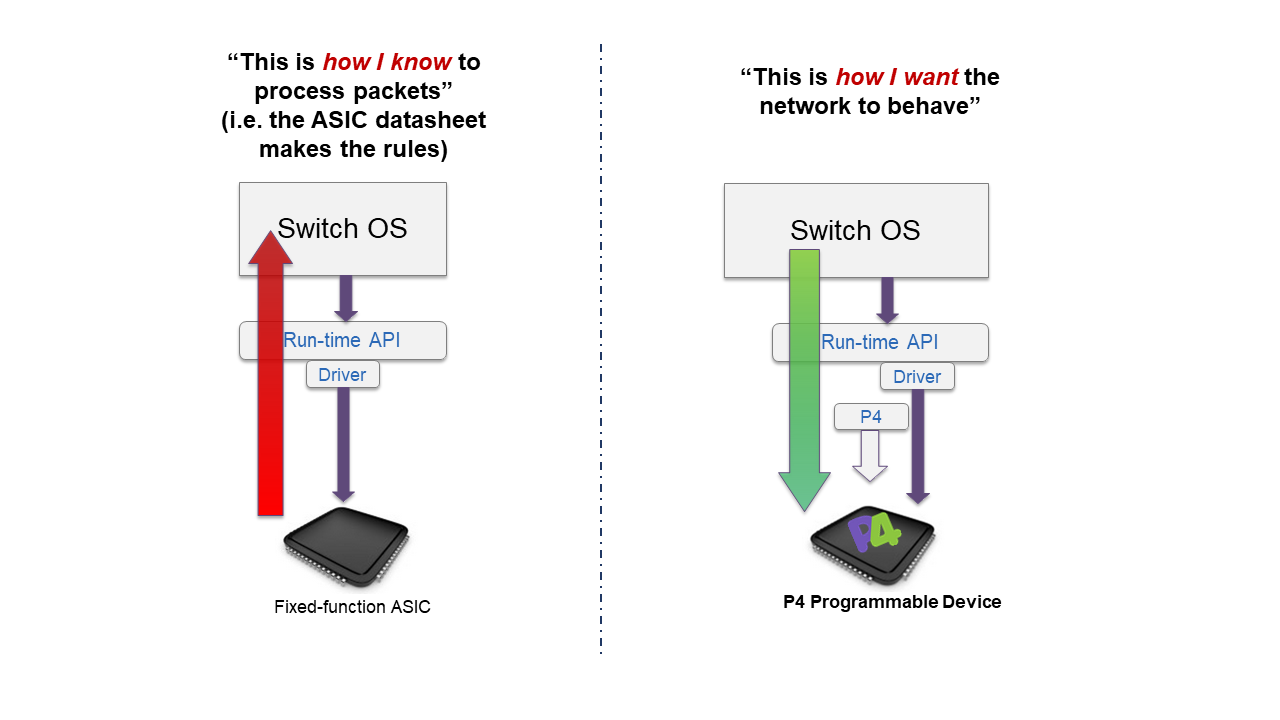
\includegraphics[width=13.5cm]{archivos/img/teoria/p4Paradigm.png}
    \caption{Cambio de paradigma con la tecnología P4 \cite{p42}}
    \label{fig:p4Paradigma}
\end{figure}


%%%%%%%%%%%%%%%%%%%%%%%%%%%%%%%%%%%%%%%%%%%%%%%%%%%%%%%%%%%%%%%%%%%%%%%%%%%%%%%%%%%
\subsection{Arquitectura y targets}

A partir de la especificación P4\textsubscript{16} se definen dos nuevos conceptos para conseguir alcanzar la independencia de los programas P4 de las distintas arquitecturas de cada fabricante. 

\begin{itemize}
    \item El concepto de \textit{Target}, se puede ver como una implementación del hardware/software especifica donde se va a correr un programa P4.
    \item El concepto de \textit{Architecture}, se puede definir como la interfaz presentada por el fabricante para programar un \textit{target} a través de componentes P4. 
\end{itemize}

% Foto 
\begin{figure}[ht]
    \centering
    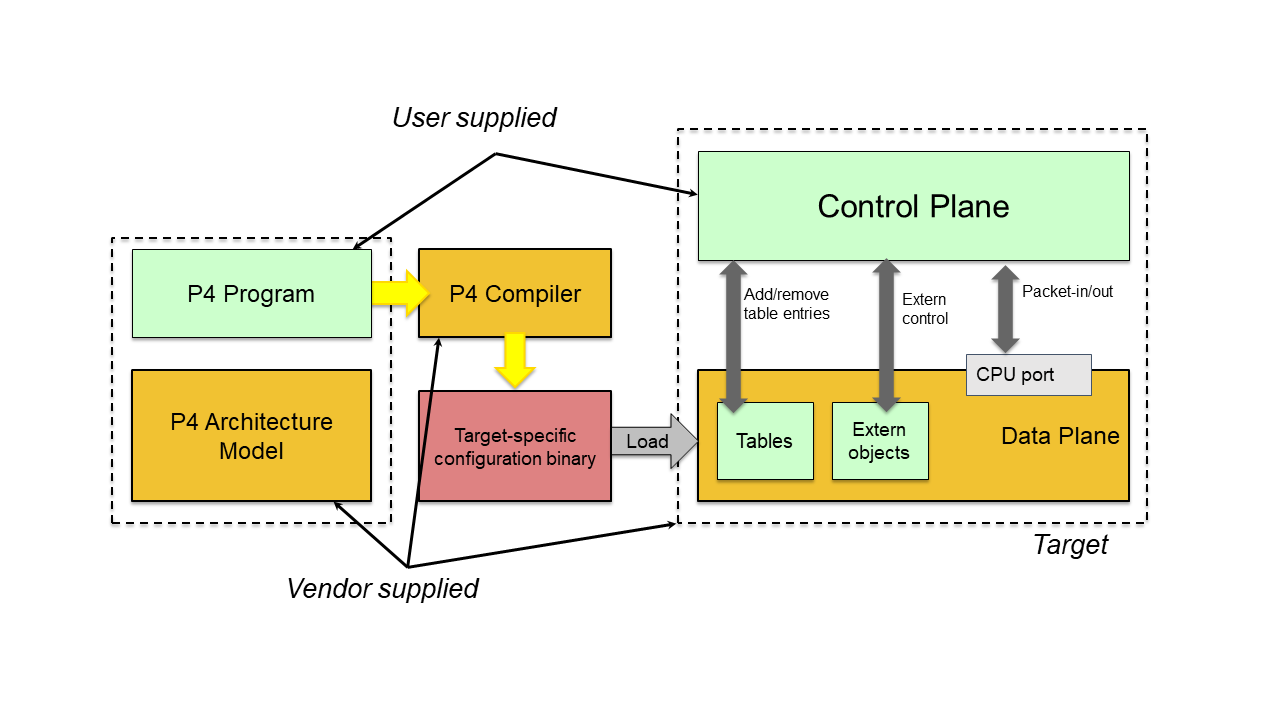
\includegraphics[width=14.5cm]{archivos/img/teoria/p4arch.png}
    \caption{Arquitectura de la tecnología P4 \cite{p42}}
    \label{fig:p4arch}
\end{figure}

Como se puede ver en la figura \ref{fig:p4arch}, el fabricante es el encargado de proveer la arquitectura, compilador y el \textit{target}. Y el usuario solo se tendrá que preocupar de escribir un programa P4 y definir la interfaz de control. De esta forma, se quiere conseguir que el usuario solo se preocupe en seguir la interfaz/arquitectura dada por el fabricante para programar un \textit{target} en especifico.\\
\par
Un programa P4 desarrollado para una arquitectura será exportable entre distintos \textit{targets} que implementen la misma arquitectura. Por lo que, si las arquitecturas como por ejemplo \texttt{v1model}, \texttt{PSA} se asientan entre los distintos fabricantes de hardware se conseguirá la independencia del hardware, para depender solo del software.  

%%%%%%%%%%%%%%%%%%%%%%%%%%%%%%%%%%%%%%%%%%%%%%%%%%%%%%%%%%%%%%%%%%%%%%%%%%%%%%%%%%%
% \subsection{Elementos del lenguaje P4}

% \begin{itemize}
%     % cabs
%     \item \textbf{Cabeceras},
    
%     % parsers
%     \item \textbf{Parsers},
    
%     % tablas
%     \item \textbf{Tablas},
    
%     % actions 
%     \item \textbf{Acciones}, 
% \end{itemize}









